% Homework 21.tex 

\documentclass{article}
\usepackage{graphicx} % for figures
\usepackage{float}
\usepackage[export]{adjustbox}
\usepackage{fancyhdr}
\begin{document}

\title{Homework 11 - Physics 240\\
		Schordinger equation}
\author{Tin Tran}

\maketitle

\section{Introduction}
The goal of this homework is to solve the Schrodinger equation using the numerical PDE methods.

\section{Discussion and data}
Belows are the plots that generated when I included the V potention for which V(x) = U$\delta$(x-L/2), whereas U can be equal to, less than, or more than E = $\hbar^2k_0^2/2m$\\\\
For U = E I got:

\begin{figure}[H]
\centering{
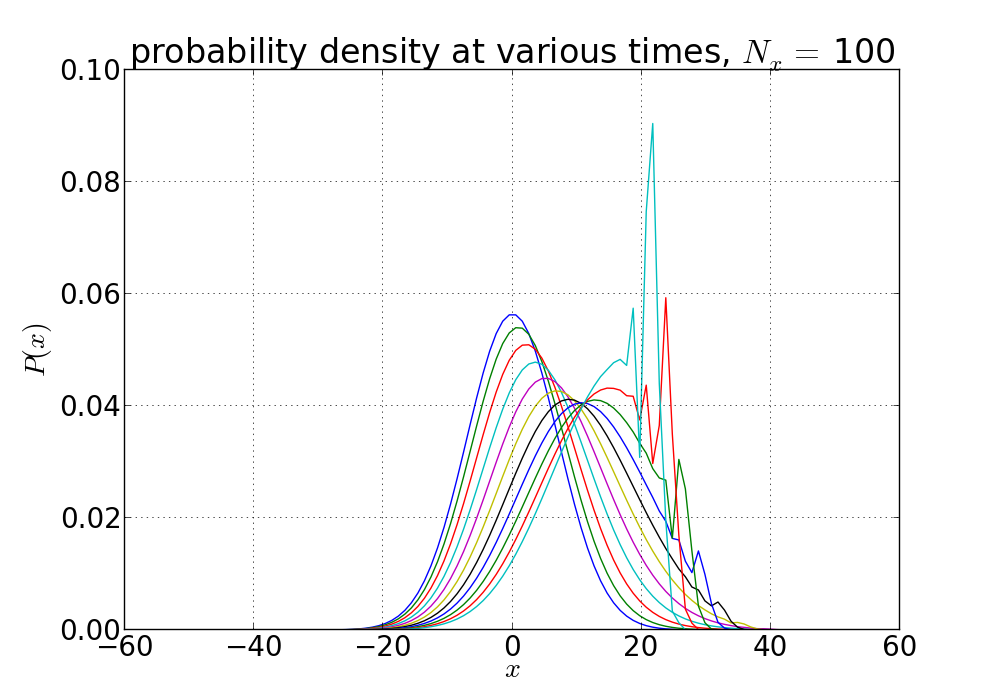
\includegraphics[max size={3 in}{4 in}]{hw21a.png}
\caption{U = E}
}
\end{figure}

\begin{figure}[H]
\centering{
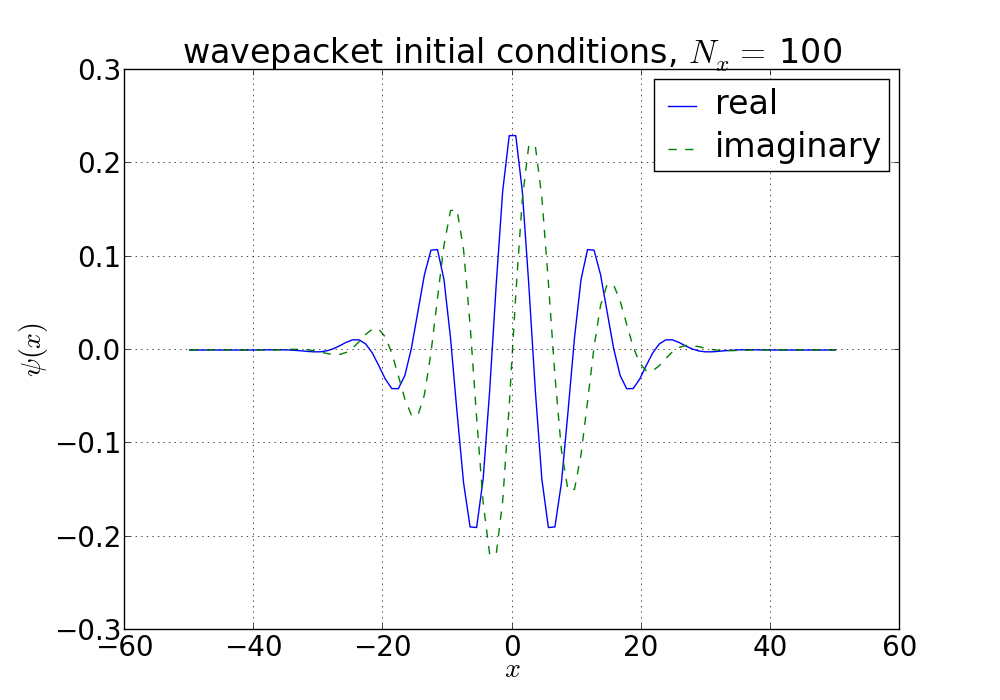
\includegraphics[max size={3 in}{4 in}]{hw21a2.png}
\caption{U = E}
}
\end{figure}

For U = 0.5E I got
\begin{figure}[H]
\centering{
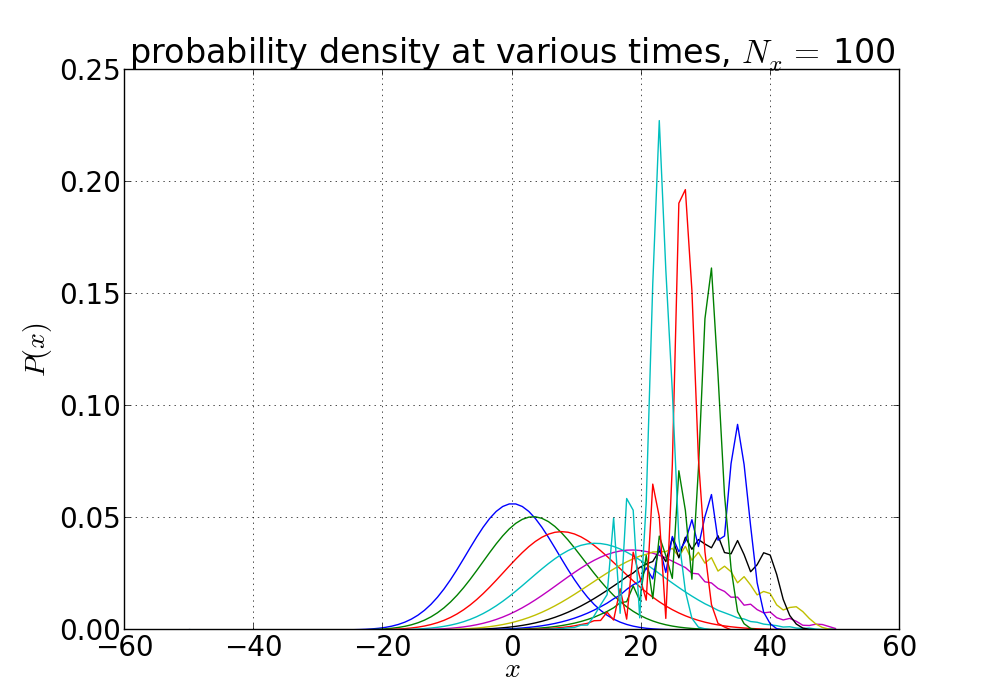
\includegraphics[max size={3 in}{4 in}]{hw21b1.png}
\caption{U = 0.5E}
}
\end{figure}

\begin{figure}[H]
\centering{
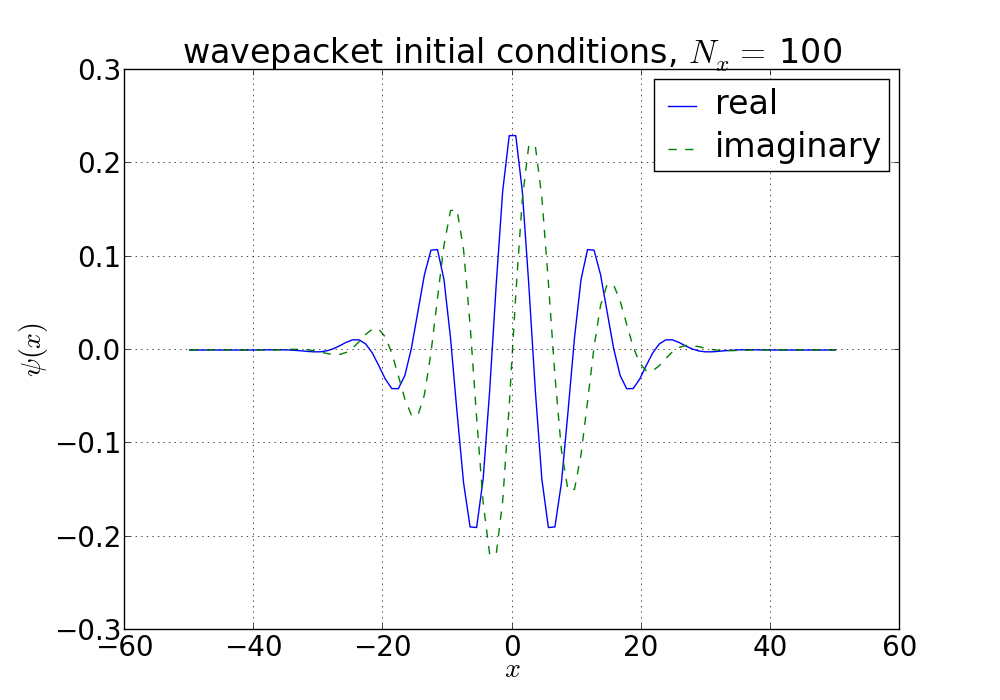
\includegraphics[max size={3 in}{4 in}]{hw21b2.png}
\caption{U = 0.5E}
}
\end{figure}

\begin{figure}[H]
\centering{
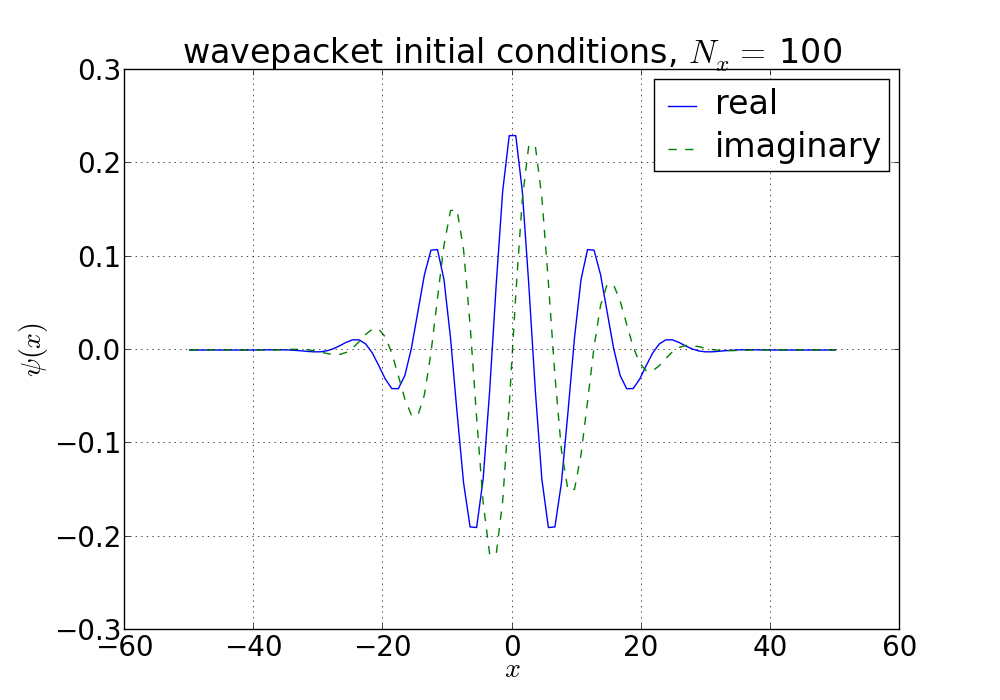
\includegraphics[max size={3 in}{4 in}]{hw21b2.png}
\caption{U = 0.5E}
}
\end{figure}

And for U = 2E I got:
\begin{figure}[H]
\centering{
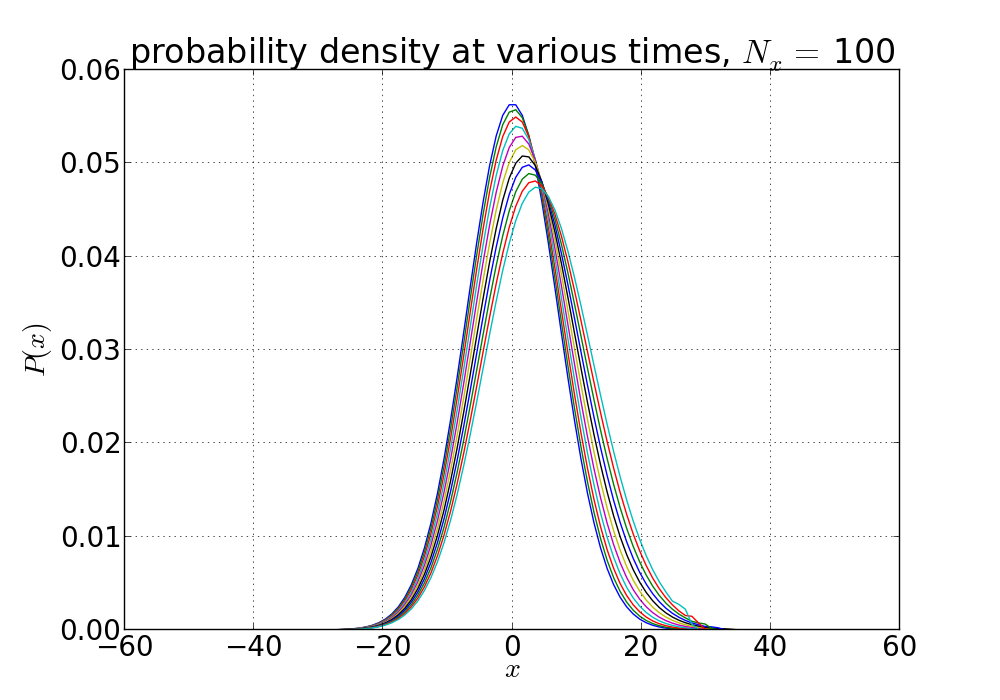
\includegraphics[max size={3 in}{4 in}]{hw21c1.png}
\caption{}
}
\end{figure}

\begin{figure}[H]
\centering{
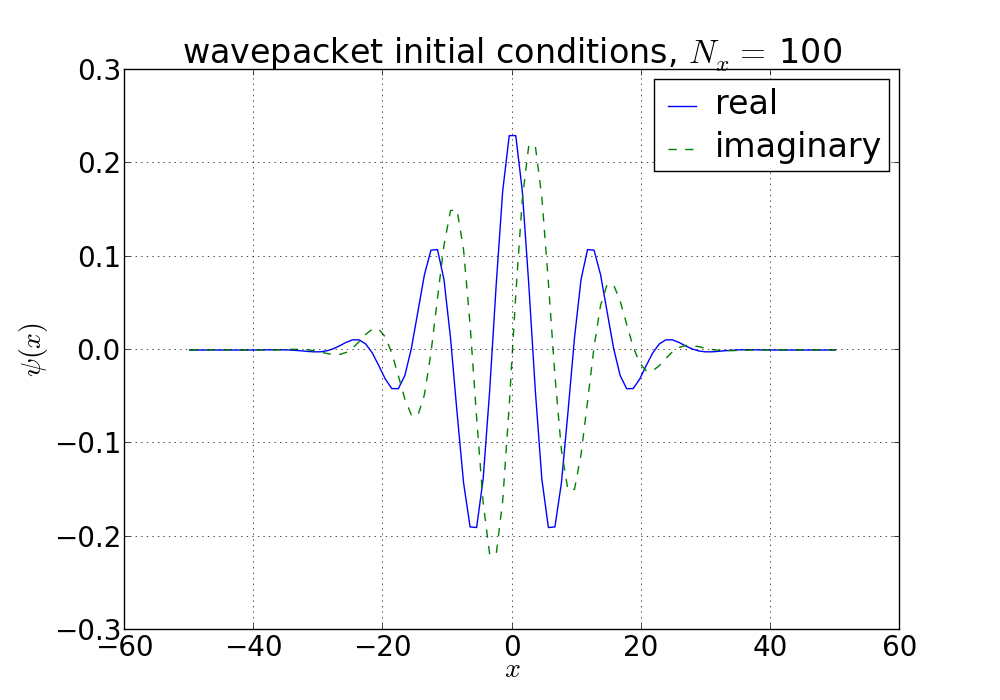
\includegraphics[max size={3 in}{4 in}]{hw21c2.png}
\caption{}
}
\end{figure}
\end{document}